%%%%%%%%%%%%%%%%%%%%%%%%%%%%%%%%%%%%%%%%%
% Wenneker Article
% LaTeX Template
% Version 2.0 (28/2/17)
%
% This template was downloaded from:
% http://www.LaTeXTemplates.com
%
% Authors:
% Vel (vel@LaTeXTemplates.com)
% Frits Wenneker
%
% License:
% CC BY-NC-SA 3.0 (http://creativecommons.org/licenses/by-nc-sa/3.0/)
%
%%%%%%%%%%%%%%%%%%%%%%%%%%%%%%%%%%%%%%%%%

%----------------------------------------------------------------------------------------
%	PACKAGES AND OTHER DOCUMENT CONFIGURATIONS
%----------------------------------------------------------------------------------------

\documentclass[10pt, a4paper, twocolumn]{article} % 10pt font size (11 and 12 also possible), A4 paper (letterpaper for US letter) and two column layout (remove for one column)

%%%%%%%%%%%%%%%%%%%%%%%%%%%%%%%%%%%%%%%%%
% Wenneker Article
% Structure Specification File
% Version 1.0 (28/2/17)
%
% This file originates from:
% http://www.LaTeXTemplates.com
%
% Authors:
% Frits Wenneker
% Vel (vel@LaTeXTemplates.com)
%
% License:
% CC BY-NC-SA 3.0 (http://creativecommons.org/licenses/by-nc-sa/3.0/)
%
%%%%%%%%%%%%%%%%%%%%%%%%%%%%%%%%%%%%%%%%%

%----------------------------------------------------------------------------------------
%	PACKAGES AND OTHER DOCUMENT CONFIGURATIONS
%----------------------------------------------------------------------------------------

\usepackage[english]{babel} % English language hyphenation

\usepackage{microtype} % Better typography

\usepackage{amsmath,amsfonts,amsthm} % Math packages for equations

\usepackage[svgnames]{xcolor} % Enabling colors by their 'svgnames'

\usepackage[hang, small, labelfont=bf, up, textfont=it]{caption} % Custom captions under/above tables and figures

\usepackage{booktabs} % Horizontal rules in tables

\usepackage{lastpage} % Used to determine the number of pages in the document (for "Page X of Total")

\usepackage{graphicx} % Required for adding images

\usepackage{enumitem} % Required for customising lists
\setlist{noitemsep} % Remove spacing between bullet/numbered list elements

\usepackage{sectsty} % Enables custom section titles
\allsectionsfont{\usefont{OT1}{phv}{b}{n}} % Change the font of all section commands (Helvetica)


%----------------------------------------------------------------------------------------
%	MARGINS AND SPACING
%----------------------------------------------------------------------------------------

\usepackage{geometry} % Required for adjusting page dimensions

\geometry{
	top=1cm, % Top margin
	bottom=1.5cm, % Bottom margin
	left=2cm, % Left margin
	right=2cm, % Right margin
	includehead, % Include space for a header
	includefoot, % Include space for a footer
	%showframe, % Uncomment to show how the type block is set on the page
}

\setlength{\columnsep}{7mm} % Column separation width

%----------------------------------------------------------------------------------------
%	FONTS
%----------------------------------------------------------------------------------------

\usepackage[T1]{fontenc} % Output font encoding for international characters
\usepackage[utf8]{inputenc} % Required for inputting international characters

\usepackage{XCharter} % Use the XCharter font

\definecolor{metblue}{RGB}{0, 86, 119}
\definecolor{metdarkblue}{RGB}{0, 65, 106}
\definecolor{metorange}{RGB}{239, 117, 33}

%----------------------------------------------------------------------------------------
%	HEADERS AND FOOTERS
%----------------------------------------------------------------------------------------

\usepackage{fancyhdr} % Needed to define custom headers/footers
\pagestyle{fancy} % Enables the custom headers/footers

\renewcommand{\headrulewidth}{0.0pt} % No header rule
\renewcommand{\footrulewidth}{0.4pt} % Thin footer rule

\renewcommand{\sectionmark}[1]{\markboth{#1}{}} % Removes the section number from the header when \leftmark is used

%\nouppercase\leftmark % Add this to one of the lines below if you want a section title in the header/footer

% Headers
\lhead{} % Left header
\chead{\textit{\thetitle \ -- Metrasens Proprietary}} % Center header - currently printing the article title
\rhead{} % Right header

% Footers
\lfoot{} % Left footer
\cfoot{Commercial in Confidence $|$ \copyright \ Metrasens Ltd. 2022} % Center footer
\rfoot{\footnotesize \textcolor{metdarkblue}{Page \thepage\ of \pageref*{LastPage}}} % Right footer, "Page 1 of 2"

\fancypagestyle{firstpage}{ % Page style for the first page with the title
	\fancyhf{}
	\renewcommand{\footrulewidth}{0pt} % Suppress footer rule
}

%----------------------------------------------------------------------------------------
%	TITLE SECTION
%----------------------------------------------------------------------------------------

\newcommand{\authorstyle}[1]{{\large\usefont{OT1}{phv}{b}{n}\color{metdarkblue}#1}} % Authors style (Helvetica)

\newcommand{\metdisclaimer}[1]{{\usefont{OT1}{phv}{m}{sl}\color{Black}#1}} % Institutions style (Helvetica)

\usepackage{titling} % Allows custom title configuration

\newcommand{\HorRule}{\color{metorange}\rule{\linewidth}{2pt}} % Defines the gold horizontal rule around the title

\pretitle{
	\begin{center}
		
\includegraphics[scale=0.8]{Figures/metrasens_horizontal_color.png}
	\end{center}
	\vspace{-30pt} % Move the entire title section up
	\HorRule\vspace{10pt} % Horizontal rule before the title
	\fontsize{32}{36}\usefont{OT1}{phv}{b}{n}\selectfont % Helvetica
	\color{metblue} % Text colour for the title and author(s)
}

\posttitle{\par\vskip 15pt} % Whitespace under the title

\preauthor{} % Anything that will appear before \author is printed

\postauthor{ % Anything that will appear after \author is printed
	\vspace{10pt} % Space before the rule
	\par\HorRule % Horizontal rule after the title
	\vspace{20pt} % Space after the title section
}

%----------------------------------------------------------------------------------------
%	ABSTRACT
%----------------------------------------------------------------------------------------

\usepackage{lettrine} % Package to accentuate the first letter of the text (lettrine)
\usepackage{fix-cm}	% Fixes the height of the lettrine

\newcommand{\initial}[1]{ % Defines the command and style for the lettrine
	\lettrine[lines=3,findent=4pt,nindent=0pt]{% Lettrine takes up 3 lines, the text to the right of it is indented 4pt and further indenting of lines 2+ is stopped
		\color{metorange}% Lettrine colour
		{#1}% The letter
	}{}%
}

\usepackage{xstring} % Required for string manipulation

\newcommand{\lettrineabstract}[1]{
	\StrLeft{#1}{1}[\firstletter] % Capture the first letter of the abstract for the lettrine
	\initial{\firstletter}\textbf{\StrGobbleLeft{#1}{1}} % Print the abstract with the first letter as a lettrine and the rest in bold
}

%----------------------------------------------------------------------------------------
%	BIBLIOGRAPHY
%----------------------------------------------------------------------------------------

\usepackage[backend=bibtex,style=authoryear]{biblatex} % Use the bibtex backend with the authoryear citation style (which resembles APA)

\addbibresource{references.bib} % The filename of the bibliography

\usepackage[autostyle=true]{csquotes} % Required to generate language-dependent quotes in the bibliography

\usepackage{hyperref}

\hypersetup{ colorlinks=true, linkcolor=metorange, filecolor=metorange, urlcolor=metblue, citecolor=metblue}
 % Specifies the document structure and loads requires packages
\usepackage{url}

%----------------------------------------------------------------------------------------
%	ARTICLE INFORMATION
%----------------------------------------------------------------------------------------

\title{State Space Modelling for Ferromagnetic Detection} % The article title

\author{
	\authorstyle{Richard Hodgskin-Brown} % Authors
	\newline\newline % Space before institutions
	\metdisclaimer{Commercial in Confidence $|$ \copyright \ Metrasens Ltd. 2022}\\ % Metrasens Disclaimer
}

% Example of a one line author/institution relationship
%\author{\newauthor{John Marston} \newinstitution{Universidad Nacional Autónoma de México, Mexico City, Mexico}}

\date{\today} % Add a date here if you would like one to appear underneath the title block, use \today for the current date, leave empty for no date

%----------------------------------------------------------------------------------------

\begin{document}


\maketitle % Print the title

\thispagestyle{firstpage} % Apply the page style for the first page (no headers and footers)


%----------------------------------------------------------------------------------------
%	ABSTRACT
%----------------------------------------------------------------------------------------

\lettrineabstract{This document aims to give a general overview of the problem of intelligent ferromagnetic detection, especially as it relates to the Metrasens product “Skout”, a passive ferromagnetic security screening device. An attempt is made to formulate a simplified version of this problem in the language of state space models, and a roadmap outlining further improvements to this simplified approach is given. A description of the different kinds of data Metrasens could supply to help with this work is also provided.}

%----------------------------------------------------------------------------------------
%	ARTICLE CONTENTS
%----------------------------------------------------------------------------------------

\section{Overview}

Metrasens are developing a new class of ferromagnetic detection systems to provide greater capability in several markets, with urban security being a particular target. The systems belonging to this new generation are designed to not only detect the presence of ferromagnetic objects, but to discriminate threat items from benign objects carried by the general population: for example, a perfect system should ignore a mobile phone but raise an alarm for an assault rifle. The wide range of benign ferrous items carried day-to-day by the public, in combination with the complex and varied nature of the potential threat items, make this a considerably difficult problem. In the simplest case, in which passive magnetometers are used to record the intrinsic ferromagnetic signature of the traversing items, there is a limited amount of information available to make this classification. Advanced signal processing and machine learning techniques are therefore being researched to enhance the performance to a satisfactory level, and it is believed that sequential Bayesian estimation techniques may be a powerful approach to this problem.

Though in principle these techniques might be applied to any of the new technologies in development, this project will focus on the application to the upcoming Metrasens product "Skout". This technology utilises a set of magnetometers to measure the magnetic field (“B-field”) passively produced by traversing ferrous objects. These can be measured over a window of time to produce a multivariate time-series (MTS), which is the basic data format that is processed by the detection algorithm.

\begin{figure}
	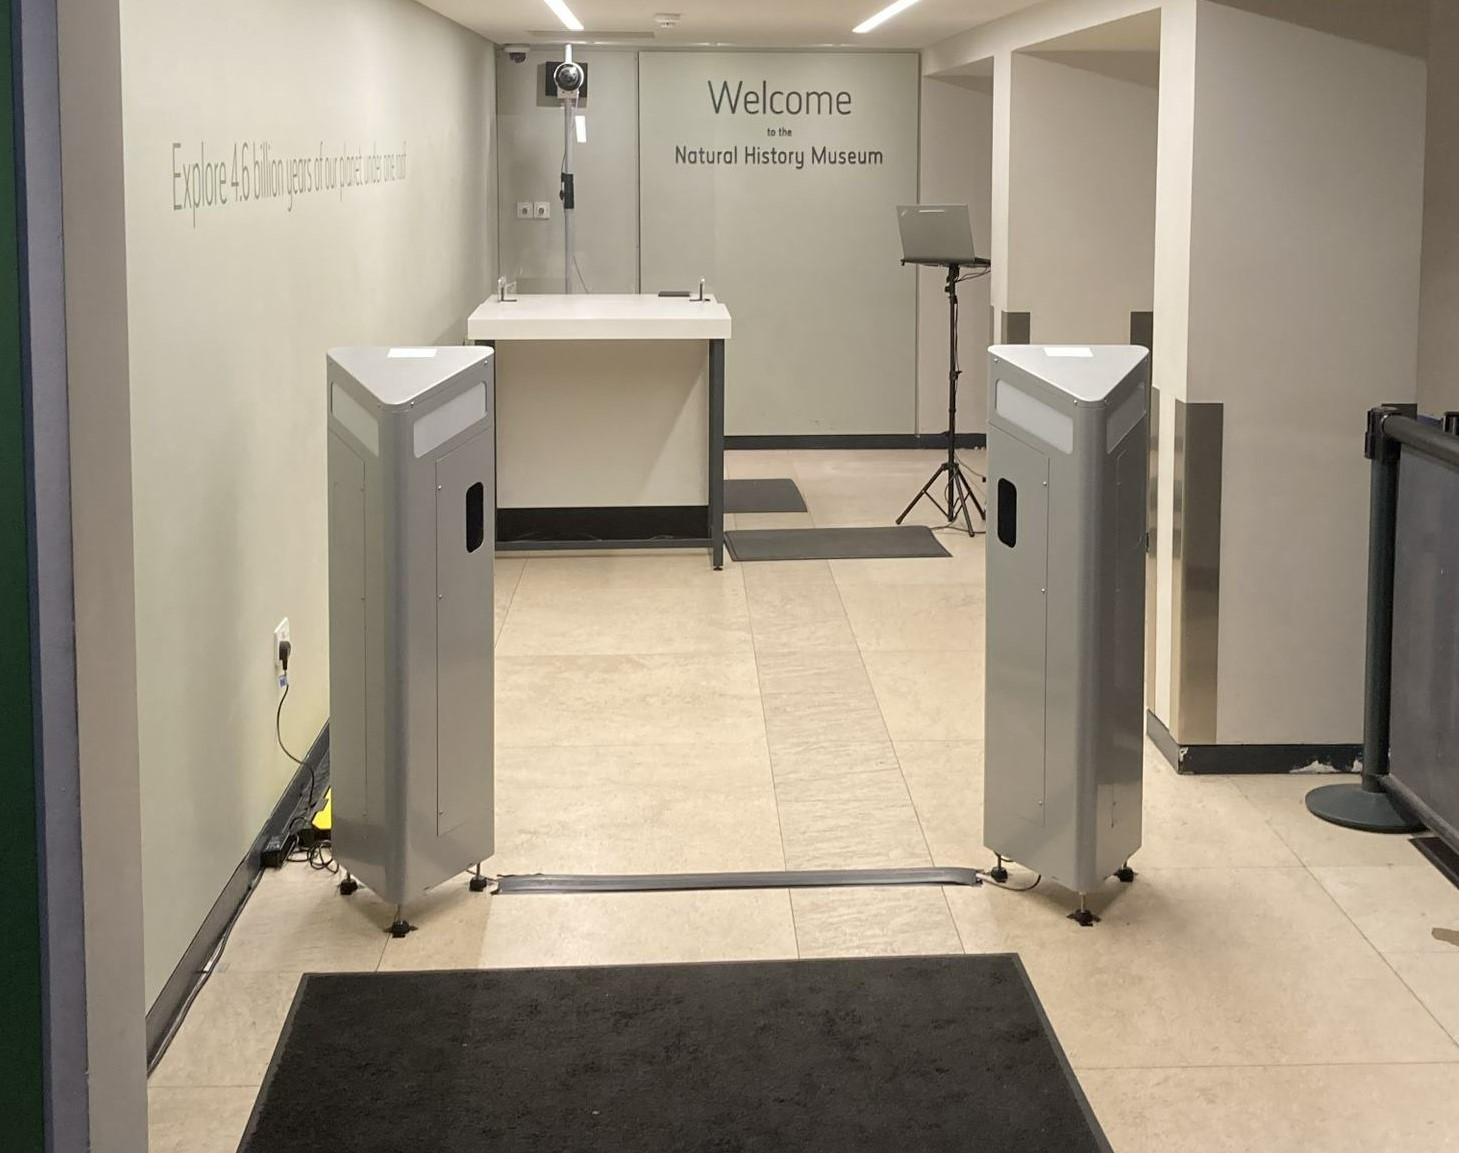
\includegraphics[width=\linewidth]{Figures/Skout_prototype.jpg} % Figure image
	\caption{Skout prototype system in deployment at the Natural History Museum to record the ferromagnetic signatures of the public.}
	\label{Skout_prototype}
\end{figure}

The basic idea for classification has been to “fit” the input MTS to a physical model, giving an intuitive, interpretable set of parameters. These parameters can then be used to make a detection decision, likely strongly incorporating anomaly/outlier detection due to the unpredictable nature of the threat set and the inherent difficulty of collecting large volumes of high-quality threat data. Including an intermediary space with interpretable parameters is believed to be crucial: only small datasets are able to be obtained, with potential heavy systematic bias in the threat sets especially, meaning that automatically learned or statistical features could be highly unreliable. Physical features help mitigate this, in theory, as only features which are intrinsic to the objects themselves (such as moment strength and object length) are sent to the classifier, and poorly understood abstract features are avoided.

The fitting step is currently being performed using the Levenberg-Marquardt technique to perform a nonlinear least squares optimisation, minimising the residuals between the recorded MTS and a simulated traversal with a given set of model parameters. Although the global minimum of the objective function is typically located correctly, this approach has a number of inherent shortcomings, which motivates the search for an improved inversion technique.


%------------------------------------------------

\section{Skout System}

This technology consists of a set of modular bollards, which we have named "pillars". The inner spaces between pillars act as channels through which the members of the public may walk, with ferromagnetic security screening performed by the pillars.

Each pillar contains six triaxial magnetometers, each capable of capturing a full three-dimensional measurement of the magnetic field (“B-field”) at a point in space. A window of data is recorded from the sensors over a range of samples, and a detection decision is made on this data: if the traversing object/s are considered to be a threat, an alarm is raised. A schematic of the Skout system\footnote{The version of this diagram used in previous correspondence incorrectly labelled the sensor separation as 15 cm; the diagram in this document is accurate.} is given in Figure \ref{Skout_schematic}.

\begin{figure}
	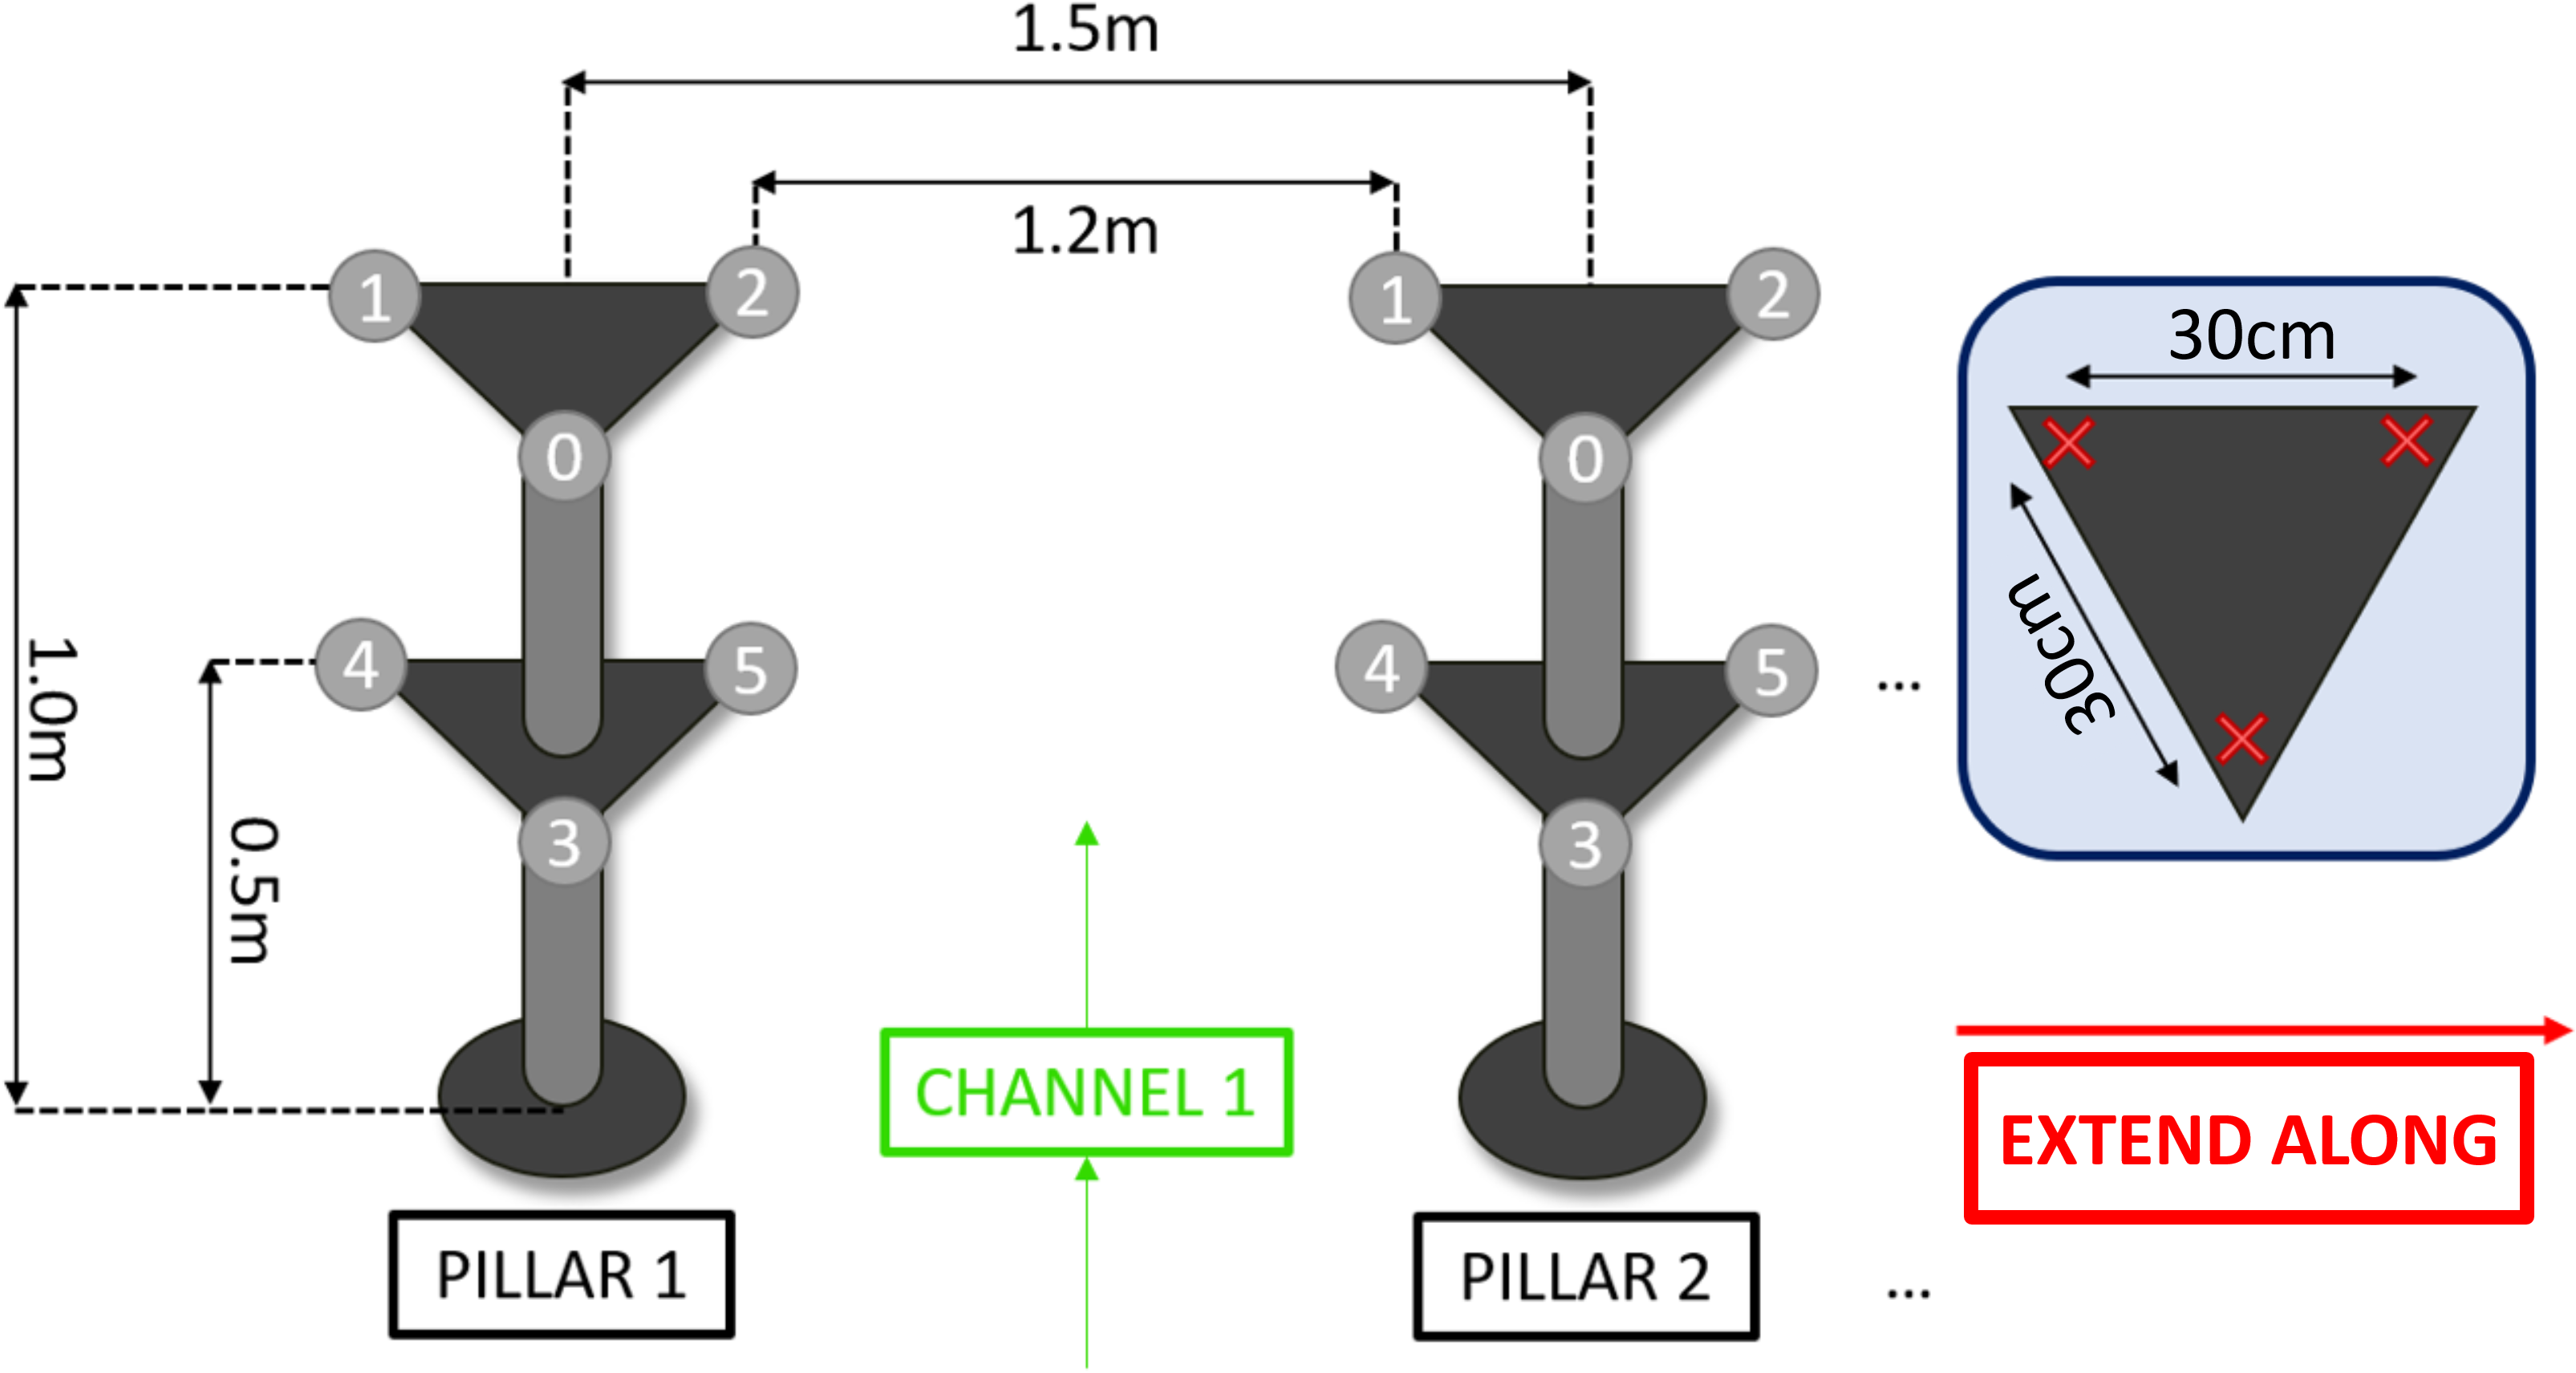
\includegraphics[width=\linewidth]{Figures/Fixed_Skout_Schematic.png} % Figure image
	\caption{A schematic diagram of the Skout system, showing all relevant dimensions.}
	\label{Skout_schematic}
\end{figure}

%------------------------------------------------

\subsection{Raw Data Format}

A Skout pillar contains six triaxial magnetometers, resulting in 18 signals per pillar (x, y, z field components are from each triaxial set are recorded separately). A channel is bordered by two pillars, so 36 magnetometer signals are recorded for a given traversal through the system. The sensors are sampled at a constant rate of 12.2 Hz, producing a 36-dimensional MTS. Currently we are considering time windows with a length of twenty samples, though this is not set in stone\footnote{This could be increased for the purposes of this investigation, but in practice there will be a fundamental limit: a window size too large will contain signals from the traversals before or after the pass in consideration.}; this produces an MTS of length 20 and width 36 (i.e. $x \in \mathbb{R}^{36\times20}$), for a total timespan of \textasciitilde1.64s. A typical window of Skout data is shown in Figure \ref{Skout_ref_data}.

\begin{figure}
	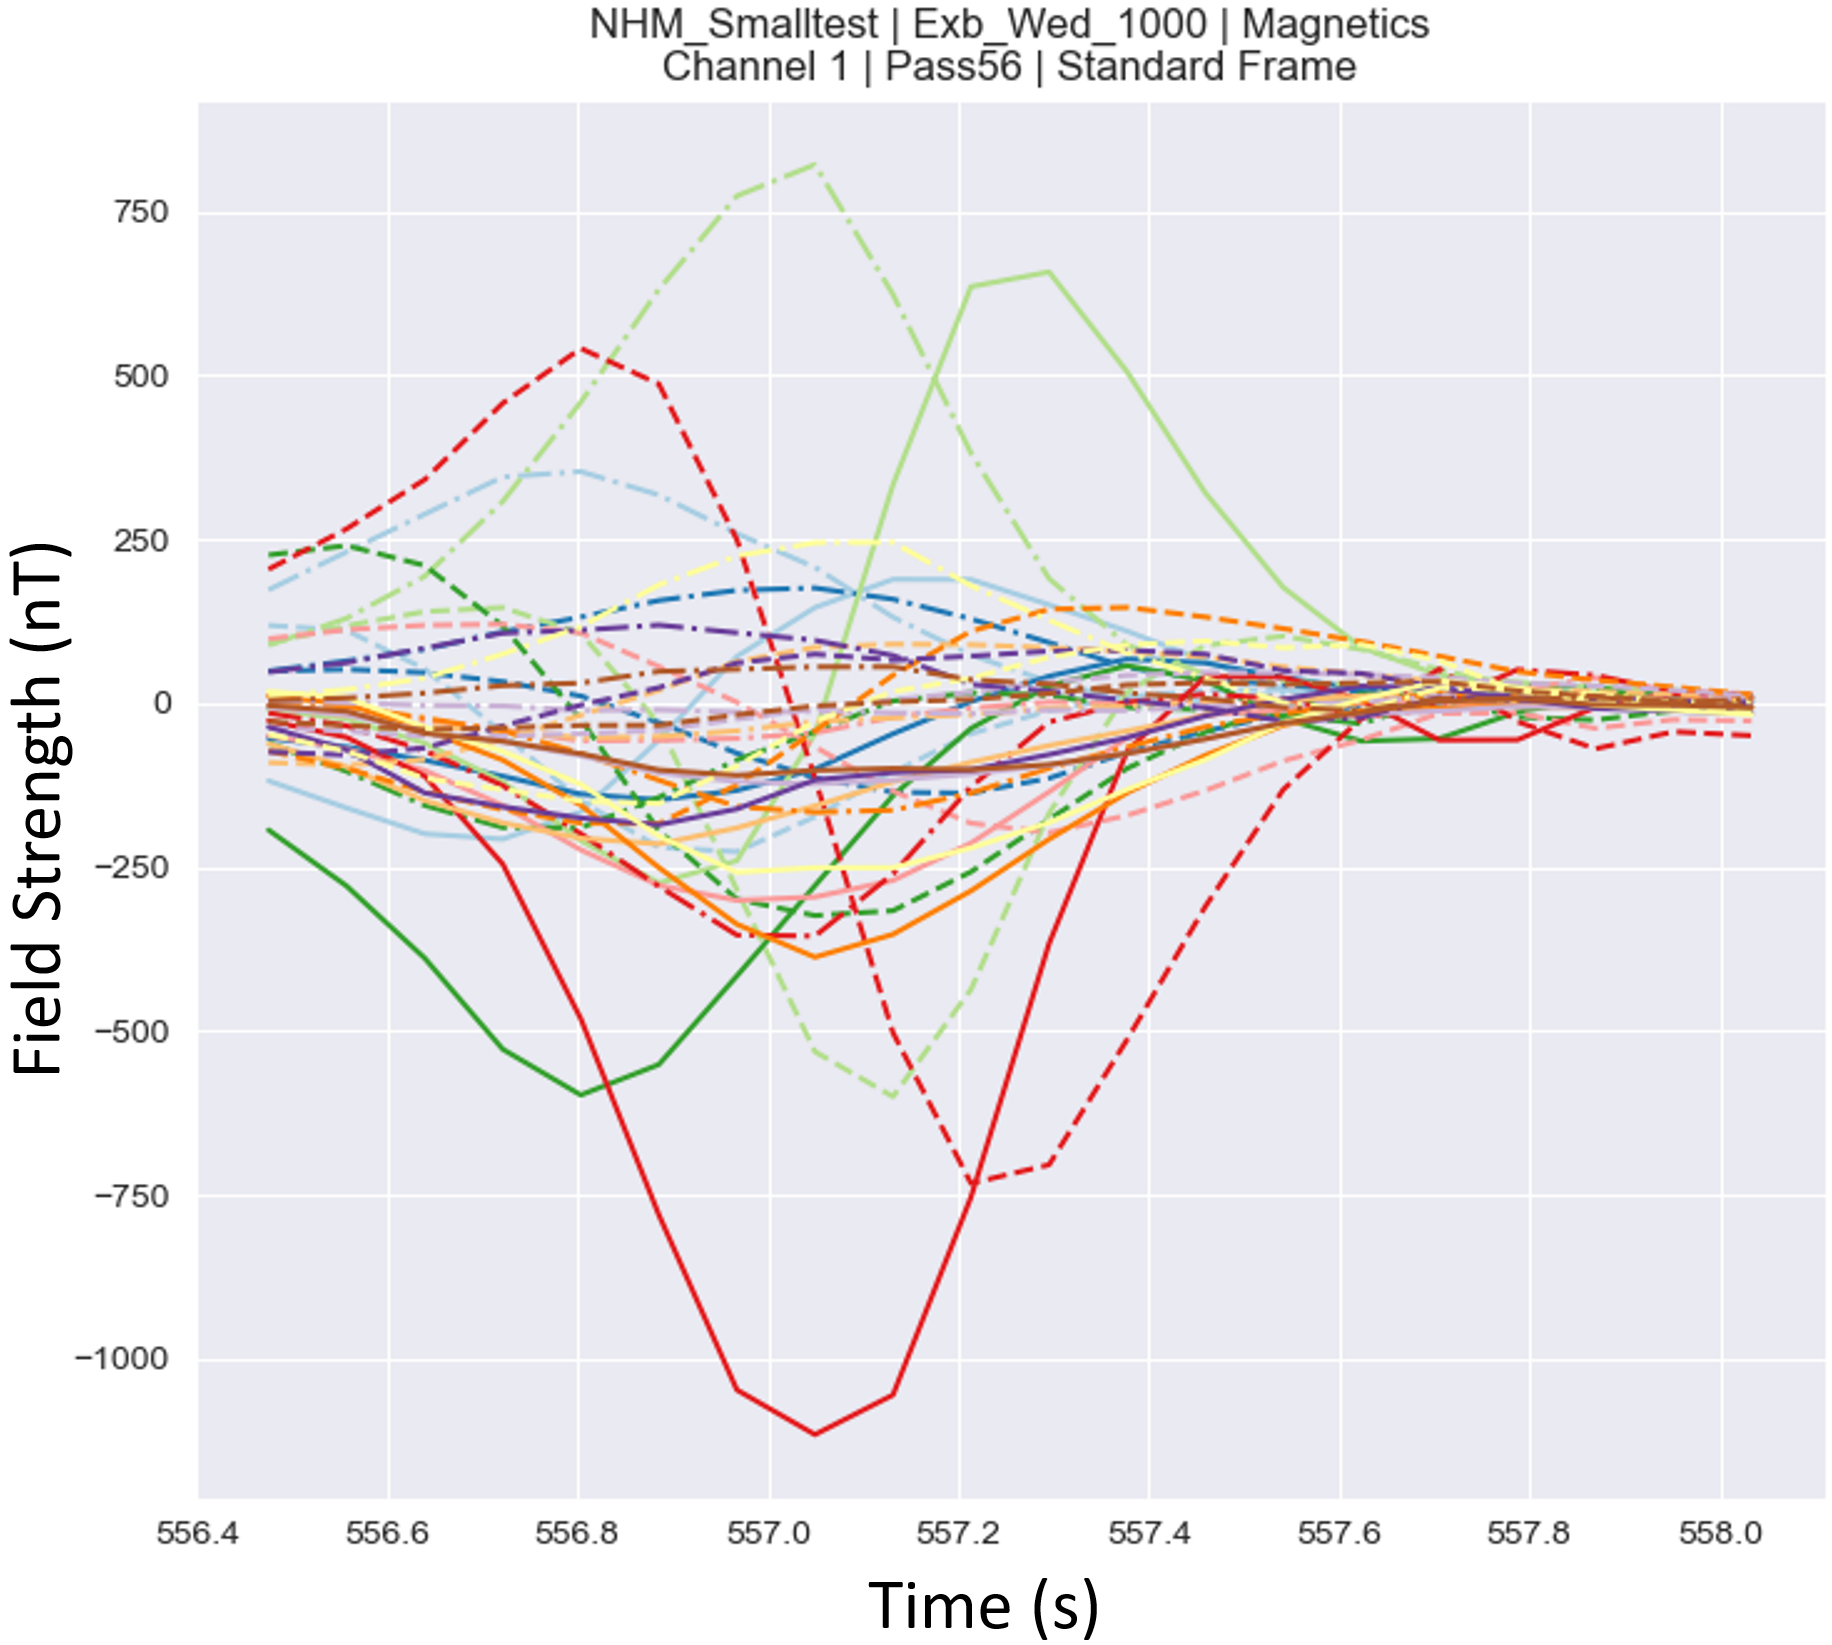
\includegraphics[width=\linewidth]{Figures/example_data.png} % Figure image
	\caption{A typical example of a Skout recording. This is a 36-dimensional time series representing the B-field measured at each sensor throughout a traversal, in this case a member of the public passing through at the Natural History Museum.}
	\label{Skout_ref_data}
\end{figure}

%------------------------------------------------

\section{Physical Model}

In the current detection paradigm, the raw data window is “fitted” to a physical model, the parameters of which are used to make a detection decision. This model is a simplified representation of what might be occurring during the traversal, informed by the physics team's domain knowledge in magnetics. In this model, a ferromagnetic object producing an idealised magnetic field travels on a specified trajectory through the Skout channel, resulting in magnetic field measurements at the sensors which change over the course of the trajectory. The field pattern at the sensors for a single time sample is dependent on three things:

\begin{enumerate}
	\item \textbf{The relative position of the ferromagnetic object and the sensors}. The magnetic field surrounding objects drops off sharply with distance, so objects located far from the sensors will produce a weaker measurement.
	
	\item \textbf{The orientation of the ferromagnetic object}. The field pattern produced by physical objects is not spherically symmetric, therefore the orientation of the object as it is carried through will affect the resultant field.
	
	\item \textbf{The magnetic properties of the object}. A more strongly magnetised object will produce a greater field measurement at the sensors. For the point dipole model, this is parameterised by the moment strength, which is the magnitude of the moment vector. More complex magnetic models may include parameters defining the size or shape of the ferrous object. See Section \ref{Mag_models} for more details.
\end{enumerate}

\subsection{Magnetic Models}
\label{Mag_models}

The simplest model of a magnetic object is the “point dipole”, a field pattern equivalent to that which would be produced by an infinitely small current loop or bar magnet. It can also be thought of as the field produced by two magnetic monopoles ("point charges") of equal and opposite charge, in the limit that the separation between them is reduced to zero (though it is worth noting that isolated magnetic monopoles do not truly exist in nature). This field pattern has cylindrical symmetry, and can be defined completely by a “magnetic dipole moment” vector (often denoted $\mathbf{m}$ or $\boldsymbol{\mu}$) which describes both strength and orientation of the dipole. The B-field produced by a point dipole source is given by the following equation:

\begin{equation}
	{\mathbf{B} ({\mathbf{r} }) = {\frac{\mu_{0}}{4\pi}} \left[{\frac {3\mathbf{r} (\mathbf{m} \cdot \mathbf {r} )}{\lvert \mathbf{r} \rvert^{5}}}-{\frac {\mathbf {m} }{\lvert \mathbf{r} \rvert^{3}}} \right],}
	\label{dipole_eq}
\end{equation}

where $\mathbf{B}$ is the magnetic field vector, $\mathbf{r}$ is the displacement between the dipole and the point being measured, $\mu_0$ is the permeability of free space (a constant),  and $\mathbf{m}$ is the magnetic moment.
The magnetic field produced by this model is plotted in Figure \ref{dipole_field}; further information can be found in \parencite{WikiDipole} and \parencite{HPDipole} in the references.

\begin{figure}
	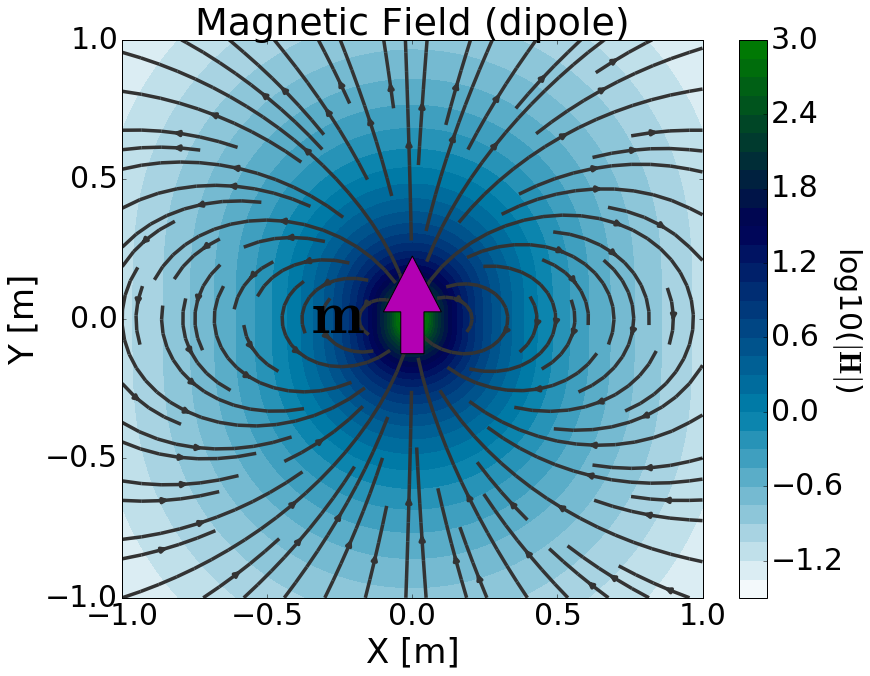
\includegraphics[width=\linewidth]{Figures/dipole_field.png} % Figure image
	\caption{This figure plots the magnetic field surrounding a point dipole which is oriented upwards. $\mathbf{H}$ is another measure of magnetic field strength, and is directly proportional to $\mathbf{B}$. Note: this is an external figure, sourced from \parencite{DefiningDipole}.}
	\label{dipole_field}
\end{figure}


A natural generalisation of this model is what we have termed the extended dipole. This consists of two magnetic monopoles with finite separation; as such, it is not strictly physical, but is a better approximation for extended ferrous objects which are not point-like in nature. This model can be described completely by a moment vector, as before, and the object “length” (i.e. the separation between the monopoles). This provides two parameters (the magnitude of the moment vector and the object length) describing the intrinsic magnetic properties of the object which can then be used for classification.

More sophisticated magnetics models are under consideration to provide additional magnetics parameters for classification. If this project is successful, a natural next step might be to augment this process with these advanced magnetic models.

\section{Current Levenberg-Marquardt Implementation}

The current detection approach uses the Levenberg-Marquardt algorithm to fit a window of data to the physical model. The following assumptions are currently made: the object follows a straight line path, remains at a constant height (i.e. the velocity has no z-component), moves at a constant speed, and does not rotate along its trajectory. An extended dipole model is used for the magnetics due to the extra parameter it provides, although our implementation can handle the point dipole case too. Figure \ref{forward_model} gives a diagrammatic representation of this model.

\begin{figure}
	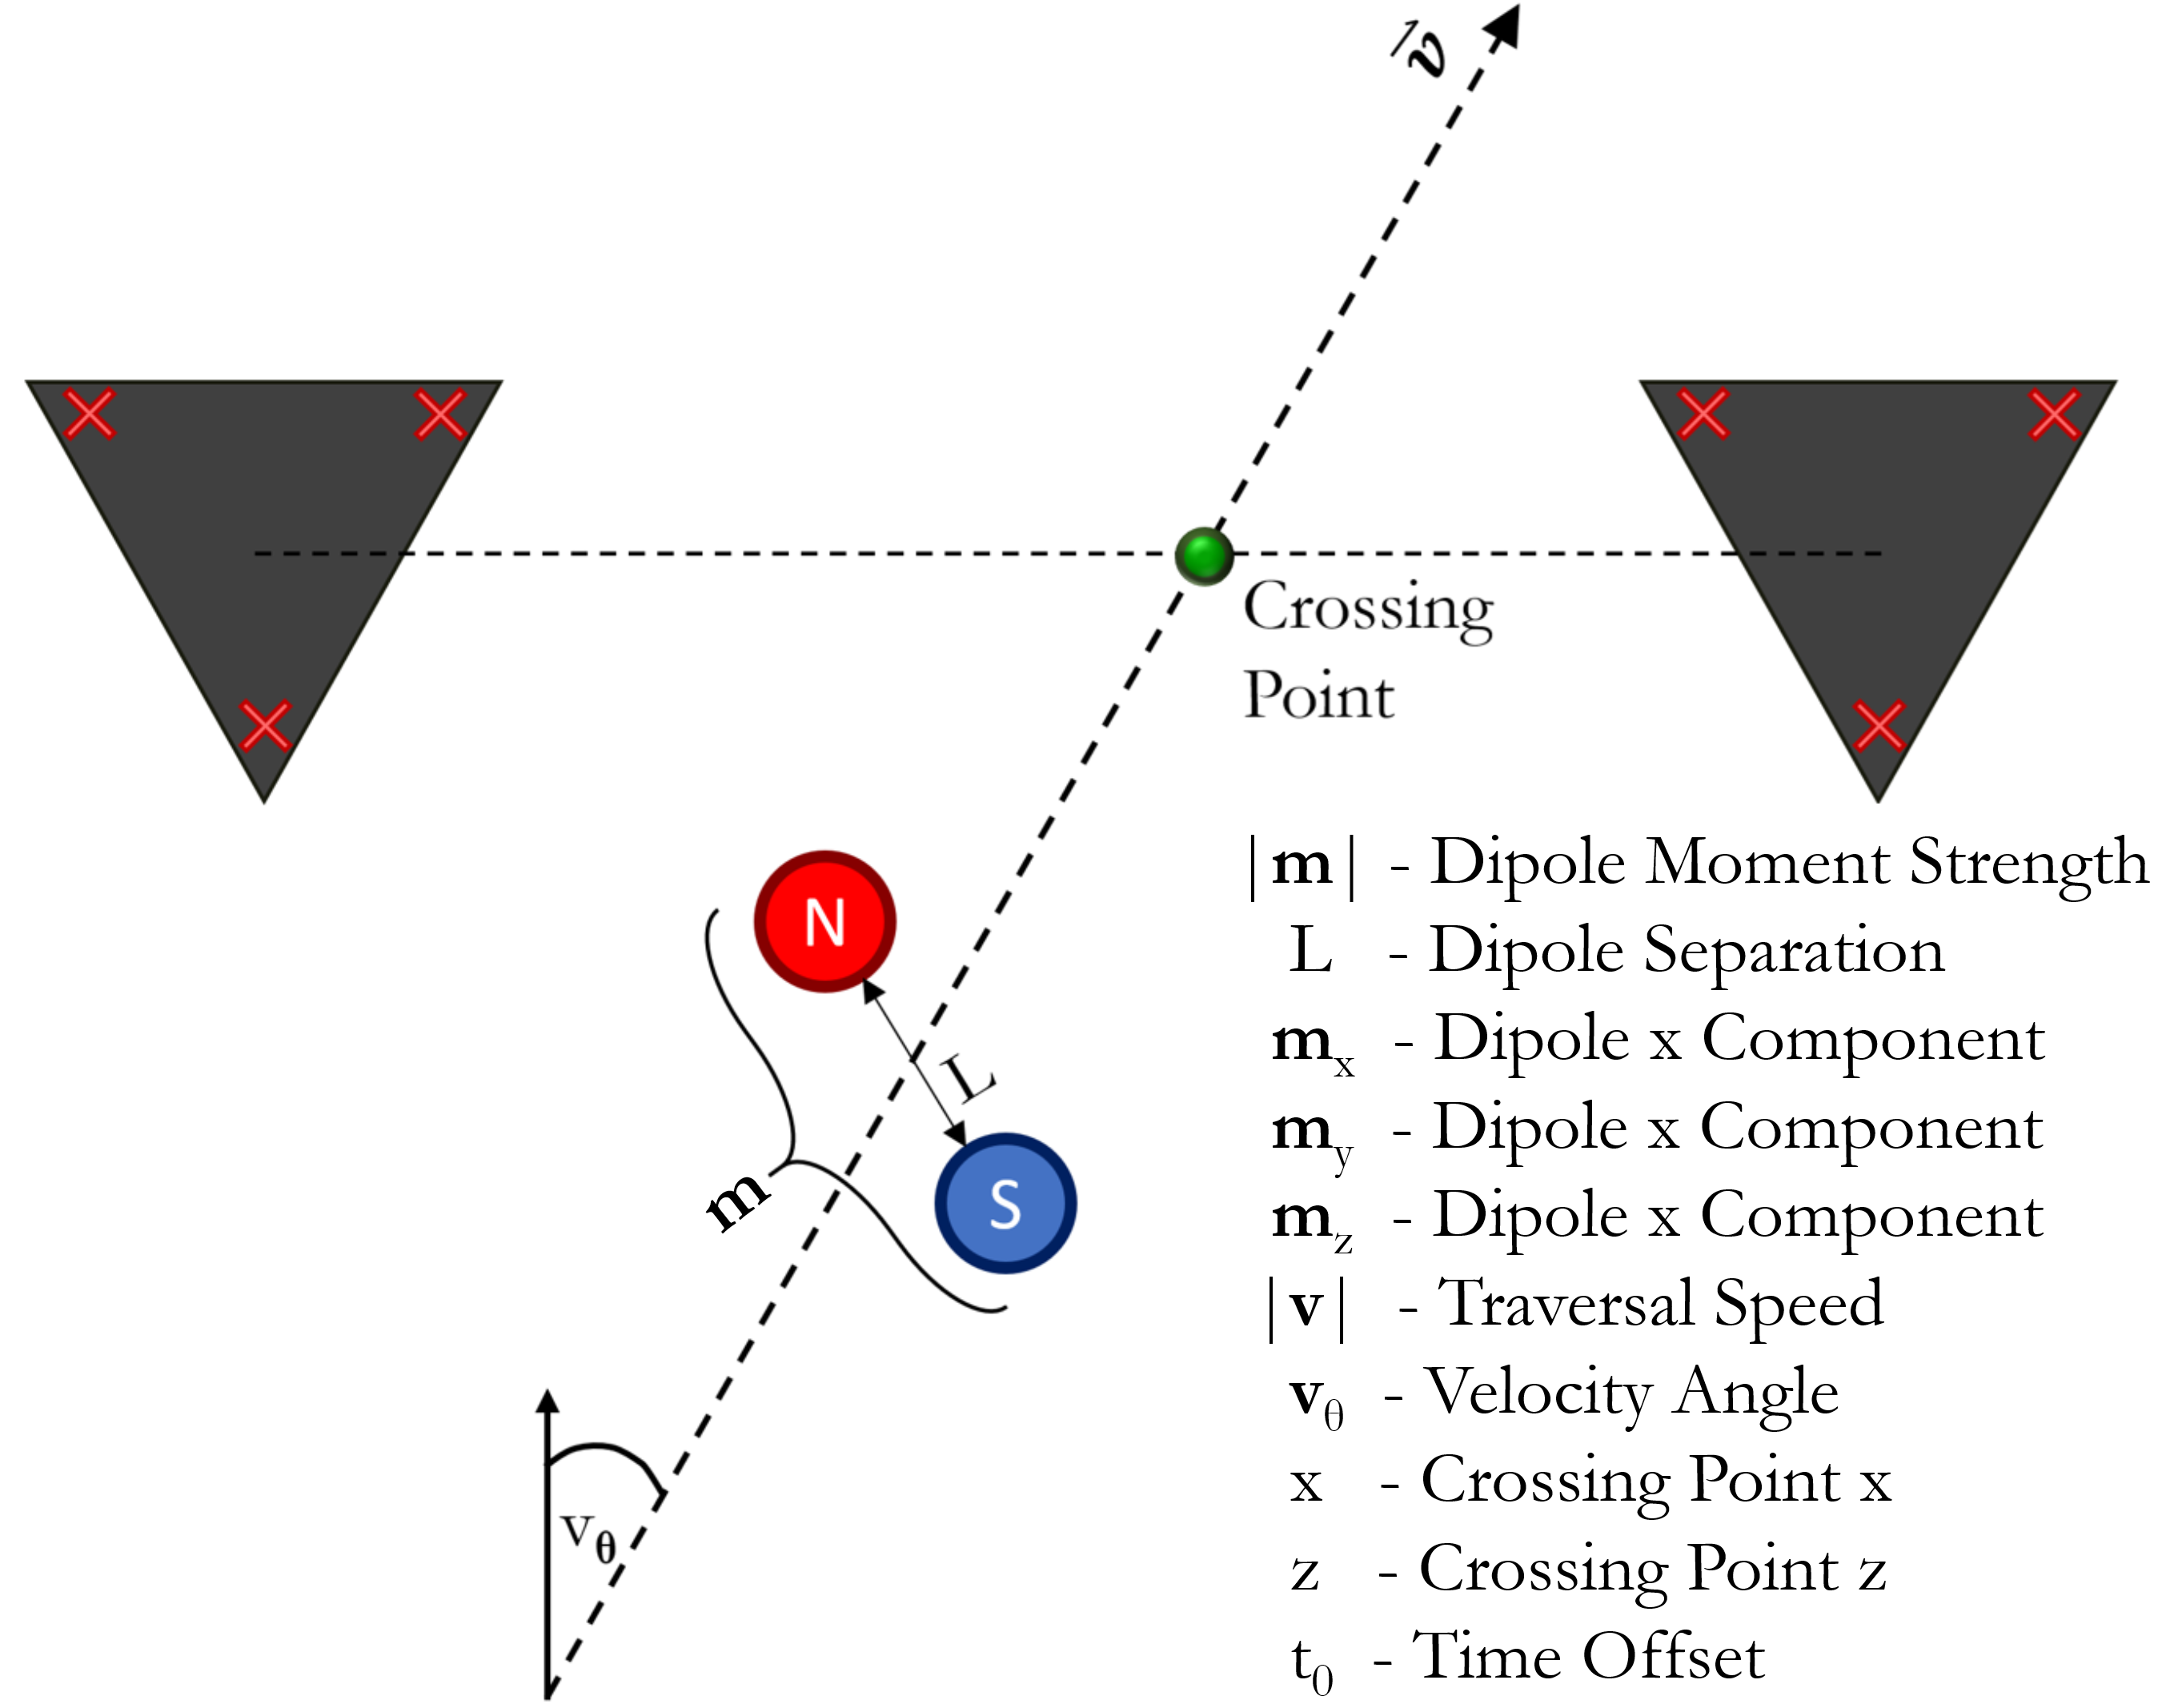
\includegraphics[width=\linewidth]{Figures/reparam_forward_model.png} % Figure image
	\caption{Model currently in use: An extended dipole, with magnetic moment strength $|\mathbf{m}|$, dipole vector components $\mathbf{m}_x$, $\mathbf{m}_y$, $\mathbf{m}_z$, and dipole separation (“length”) $L$, traverses the channel with speed $|\mathbf{v}|$, velocity angle $\mathbf{v}_\theta$, and time offset $t_0$, intersecting the sensing plane at a crossing point with dimensions $x$, $z$.}
	\label{forward_model}
\end{figure}

The physical model provides a simulation of the magnetic field at the sensors recorded over the length of a window. The squared error between this simulation and the recorded data is used to define a cost function, which is highly nonlinear with no known analytic derivative. This is therefore a nonlinear optimisation problem, and the Levenberg-Marquardt algorithm is used to find the global minimum. Sixty start-points carefully chosen across the parameter space are used to ensure the located minimum is the global rather than local minimum – in practice, this has proven to be robust for our problem, and the global minimum is typically found.

\subsection{Weaknesses of the Current Approach}

Our implementation of the Levenberg-Marquardt algorithm works as intended: the global minimum of the cost function is located. The shortcomings arise due to the inherent limitations with formulating the problem in this manner. In particular:

\begin{itemize}
	\item The current problem formulation contains very strong assumptions about the traversal trajectory: straight line, constant velocity, no orientation changes, etc. This is clearly a big oversimplification, as objects carried by human beings during a typical walkthrough will have many accelerations and deviations in the trajectory. It is also incapable of dealing with sloped surfaces and stoppages.
	
	\item There is no easy way to include prior information about the distribution of the model parameters. Currently this is being done by editing the cost function to impose sensible limits on the fitted parameters, but this is clunky and ignores detailed information about the  prior distributions that is already known.
	
	\item The end result of the fit is a point estimate of the optimum model parameters. A probability distribution over the model parameters would provide greater interpretability and more information which can be sent to the classifier\footnote{A full distribution over the model parameters would incorporate very nicely into our current anomaly detection approach.}.
\end{itemize}

It is possible that the trajectory errors might be diminished by adopting a sequential fitting approach with Lev-Mar, however for many time samples there is not enough information to get a reliable fit in a noisy environment. In addition, the strong correlations between samples is ignored with this approach, and information from the fit of one sample can not easily be utilised to influence the fit of the next. For this reason, we are hopeful that a sequential Bayesian approach might overcome the inherent shortcoming of our current fitting technique.

\section{State Space Formulation}
\label{State_space}

Our problem is well-suited to description with the language of state space models. We have a hidden state, which describes the magnetic properties, orientation, position, and velocity of the object at a given time sample, and a transition model, which updates the position of the object between samples and is a function of the state. The measurement model is given by the sensor B-field measurements at each position in the pillar, and is again a function of the state.

To demonstrate a proof of principle with this approach, it might be best to avoid excess complexity at first. A good place to start might be with a point dipole, straight line trajectory model. In this case, our problem might be formulated like this\footnote{Many different notational conventions exist for these parameters. An attempt has been made to standardise them in this document, consequently, there may be some differences with previous correspondence and cited materials.}:\\

\textbf{State vector}:

\begin{equation}
	\mathbf{x}_t = (\lvert \mathbf{m} \rvert, m_\theta, m_\phi, p_x,
	p_y, p_z, \dot p_x, \dot p_y)^T,
\end{equation}

where $\lvert \mathbf{m} \rvert$, $m_\theta$ and $m_\phi$ describe the moment vector in spherical coordinates; $p_x$, $p_y$ and $p_z$ are the x, y and z coordinates of the dipole; $\dot p_x$ and $\dot p_y$ are the x and y velocities of the dipole.\\

\textbf{Transition model}:

\begin{equation}
	f(\mathbf{x}_{t-1}) = \begin{pmatrix}
		1 & 0 & \Delta t & 0\\
		0 & 1 & 0 & \Delta t\\
		0 & 0 & 1 & 0\\
		0 & 0 & 0 & 1
	\end{pmatrix}
	\begin{pmatrix}
		p_x \\
		p_y \\
		\dot p_x \\
		\dot p_y \\
	\end{pmatrix},
	\label{simple_transition}
\end{equation}

where $\mathbf{x}_{t-1}$ is the state vector of the previous sample, and $\Delta t$ is the time between samples (1/12.2 seconds).\\

The \textbf{measurement model} is a little more complex, as it is a function of both the state vector $\mathbf{x}_t$ and the location of each sensor $\mathbf{s}_i$. If we define $\mathbf{r}_i = \mathbf{s}_i - \mathbf{p}$, where $\mathbf{p}$ is the location of the dipole in the measurement frame, then we can use Equation \ref{dipole_eq} to calculate the 3-dimensional B-field at each sensor location:

\begin{equation}
	\mathbf{y}_{t}^{i} = g(\mathbf{x}_t,\mathbf{r}_i) = {\frac{\mu_{0}}{4\pi}} \left[{\frac {3\mathbf{r}_i (\mathbf{m} \cdot \mathbf{r}_i )}{\lvert \mathbf{r}_i \rvert^{5}}}-{\frac {\mathbf {m} }{\lvert \mathbf{r}_i \rvert^{3}}} \right].
\end{equation}

The components of $\mathbf{y}_t^i$ give us the x, y and z components of the B-field at one of 12 sensor locations that constitute a channel. The full measurement vector $\mathbf{y}_t$ can therefore be obtained by concatenating the components from each sensor:

\begin{equation}
	\mathbf{y}_t = (\mathbf{y}_t^0, \mathbf{y}_t^1, \ \ldots \ , \mathbf{y}_t^{12})^T,
\end{equation}

resulting in one 36-dimensional measurement vector for each time sample.\\

The measurement model is clearly nonlinear, and will become even more complex if a more sophisticated magnetic model is used. The prior distributions for the model parameters are not necessarily Gaussian, for example, the measured benign moments appear to more closely match a lognormal distribution, and multiple modes are a possibility. Consequently, a simple Kalman filter is insufficient for our problem. We are also somewhat computationally constrained, as any solution will eventually have to run in real-time on embedded hardware. The AKKF method therefore appears a promising fit for our purposes.

It is important to note that the critical model parameter that needs to be estimated is the moment strength (along with any other parameters describing the intrinsic magnetic properties in more complex magnetic models), as this is what the detection decision will be based on. In the simplest case this is constant along the trajectory, so there is no requirement to perform any kind of real-time tracking. A full window of data can therefore be used to perform the parameter estimation, making this a smoothing problem rather than a filtering problem using the terminology defined by \parencite{Briers2009}. As only a small subset of the state parameters are necessary for classification, the other parameters might then be marginalised out (though in this case, it would be useful to store these distributions prior to marginalisation, as they have scientific utility separate from their usefulness in classification).

\section{Adding Complexity}

If we successfully verify the simple model described in Section \ref{State_space}, we can think about adding complexity to our model to improve its performance on real datasets. There are many different forms this could take, some of which are listed below.

\subsection{Key Features}

The following alterations are thought be critical for progressing past the simplistic case to achieve the performance necessary for the product:

\begin{itemize}
	\item \textbf{Advanced magnetic models}: The point dipole model only provides one useful parameter for classifying the objects, which is the dipole moment strength. Experience tells us that this is not enough to successfully discriminate threat and benign objects. The current Lev-Mar implementation uses an extended dipole model, which provides an extra “length” parameter which can be sent to a classifier, so this would be a natural next step. More sophisticated magnetic models are under consideration, but are primarily in the research stage at the moment. See Section \ref{Mag_models} for more details.
	
	\item \textbf{Improved transition model}: One of the major perceived strengths of this approach is its ability to handle more complex and unpredictable object trajectories. As such, it would be highly beneficial to add complexity to the transition model to move beyond straight-line, constant velocity trajectories. A good place to start might be the random accelerations model, in which an additional (Gaussian) noise term is added to each position and velocity parameter in Equation \ref{simple_transition}. Other augmentations, such as allowing the objects to rotate, may also add value.
	
\end{itemize}

\subsection{Advanced Features}

Time-permitting, there are several other more complex additions which could significantly improve the accuracy of the model:

\begin{itemize}
	\item \textbf{Signal differences}: One of the challenges passive detection systems face is dealing with magnetic interference from distant sources. Signals from distant objects have the characteristic that the “common-mode” component of the signal (that which appears on all sensors simultaneously) is much greater than the differences between signals. For this reason, we typically fit our models to the differences between signals rather than the raw signal itself, in effect using the system as a gradiometer. Replicating this process in the measurement model could considerably improve the performance in a real-world scenario.
	
	\item \textbf{Multiple object models}: An unfortunate reality when screening the public using this technology is that people often carry multiple ferrous objects, for example, someone might carry a phone in their pocket whilst also wearing headphones. In this scenario, a single object fit will produce unreliable results. Augmenting the state to describe multiple objects might therefore improve the quality of information sent to the classifier.
	
	\item \textbf{Interference sources}: Urban environments contain many sources of magnetic interference: traffic, subways, electrical equipment and nearby members of the public, to name just a few. Robustness against this type of interference could be critical in achieving the level of performance necessary for this technology to work effectively. It might be possible to change the model to include basic interference sources to combat this.
	
	\item \textbf{Signal processing}: The raw signals from the magnetometers are not used directly in the detection algorithm; some signal processing procedures are applied. The most important is probably the application of a high-pass filter, which removes drift in the sensors and offsets due to changes in the magnetic background. The filtering process also distorts the signals, however, which may lead to less accurate parameter estimation. It is proposed that this might be mitigated by incorporating the filtering process (or other preprocessing procedures) into the model: the state could contain extra parameters corresponding to the state of the filter at each timestep, and the measurement function would contain an extra procedure to apply the filtering process to the measured signals.
\end{itemize}

\section{Data}

Metrasens can provide a great deal of data to assist with this project. We have working simulators in Matlab and Python, covering a range of models, which can be used to provide simulated data to verify the implementation with a known ground truth. The real test for this method, however, will be its performance on genuine data recorded by the Skout system.

These recordings could cover a range of scenarios. We can record controlled traversals, using test objects with known magnetic properties, constrained to accurate straight-line trajectories using a non-magnetic trolley system. We can also record data with more realistic traversals to verify that we can cope with this scenario using more complex trajectory models. If the method is showing promise, we can evaluate its use on real Skout recordings taken during public screening data collection events. This is very messy, noisy data which is the gold standard for any detection algorithm we might try.

%----------------------------------------------------------------------------------------
%	BIBLIOGRAPHY
%----------------------------------------------------------------------------------------

\printbibliography[title={References}] % Print the references, section title in curly brackets

%----------------------------------------------------------------------------------------

\end{document}
